%% ----------------------------------------------------------------
%% Authoring.tex
%% ---------------------------------------------------------------- 
\chapter{Authoring Tool} 
\label{Chapter:Authoring Tool}
An accessible \gls{authoring} was required to allow users to create their own question sets. Within the authoring tool users can create polls and quizzes and overlay them at chosen locations in a video. This avoided the necessity for users of the framework to learn the javascript quiz schema, thus significantly reducing the technical barrier to entry. 

One key consideration during the implementation of the authoring tool was accessibility. The WCAG 2.0 guidelines were kept in mind at all times and adhered to as much as possible.

Care has been taken to ensure that the authoring tool can be easily used within other angularJS projects, and thorough documentation has been provided to ease this process.

\section{Design} 
\label{Section:Design}

Within the authoring tool users have the ability to create questions sets within a video. There could be any number of questions in a set and these could be of many different types. A range of options are given to modify the functionality of each question so as allow the user to create exactly what they need.

At any point the user can preview the quiz they have created on the inbuilt video player. Once they are satisfied with the quiz they can export it for use with videogular-questions externally from the tool.

It was decided to use Bootstrap\footnote{\url{https://github.com/twbs/bootstrap/}} to give a consistent appearance to all of the user interfaces components within the project. This is a HTML, \gls{CSS}, and JavaScript framework for developing webpages.

As an Angular framework is used, any additional functionality is required to be written as directives and controllers. UIBootstrap\footnote{\url{http://angular-ui.github.io/bootstrap/}} provides some Bootstrap components written in \gls{AngularJS}. This provides some of the components required. 

Wireframes were created using this style so that they could easily be directly coded as static HTML to allow a quick demo to be created. 

Two different approaches were suggested for showing the advanced options for the video. A pop up approach hid these from general view to avoid confusing users with lots of options that may be unnecessary. The other approach was to use the accordion structure as we had for the questions. This would be collapsed by default so the options would still be hidden. This was chosen as it was more consistent with the rest of the tool. Wireframes were created to allow for feedback from users and the customer. They can be found in \autoref{Chapter:Authoring Tool Wireframes};
\todo{Is this true anymore?}

\section{Implementation}
\label{Section:Implementation}
Once the wireframes were drawn up they could be turned into static HTML. Elements of this webpage were then incrementally given the functionality they required. The main challenge was ascertaining how the functionality fitted in with the \gls{AngularJS} Framework. 

Each section of the page had to have its own directive so that independent behaviours could be achieved. This kept the HTML pages short and readable as the behaviour was dealt with by the JavaScript and the styling dealt with by the \gls{CSS}.

Angular allowed the dynamic nature of the data to define the appearance of the page. Sections could be set to appear only when certain attributes were set using ng-switch statements. This meant one section could potentially show many different elements depending on what was selected elsewhere on the page.

\subsection{Data Bubbling}

With the authoring tool we have leveraged the ability to use two way binding and watches with AngularJS. This allows us to template a number of reusable elements such as the time picker and means we don't have to rewrite the class each time we wish to use it. This has reduced the time taken to produce the authoring tool.

The root controller holds the global state of the authoring tool. This global state is updated by the child controllers who each own specific parts of the global model. This bubbling of data up the controllers is the key to how the authoring tool has been built.

The preview and generation features utilise this model in the root controller composed from the bubbled models over the child controllers.

\begin{figure}[h]
	\centering
		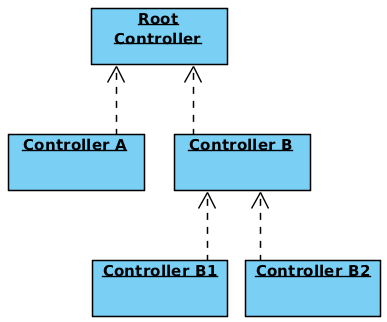
\includegraphics[scale=0.4]{../figures/authoring_tool/controller_bubbling.png} 		
	\caption{\label{Figure: Bubbling model data} Bubbling of model data up controllers} 	
\end{figure}

\autoref{Figure: Bubbling model data} shows the general structure of the controllers and how we have implemented the bubbling up of data. In our implementation we have a large number of controllers and levels to encapsulate the different ways of quiz creation. In this diagram controller A and B will bubble their model data up to the root controller if it changes. If model data in controller B1 or B2 changes, their new model will bubble up to controller B. Controller B will then will then bubble its model combined with the new model data it has received to the root controller.

This bubbling technique works for any number or levels of children provided the model data is correctly bubbled up each layer. It also makes adding new controllers at any point simple as you only need to handle the bubbling of the data up the levels.

Each controller may have one or more children who may or may not hold model data.

\begin{figure}[h]
	\centering
		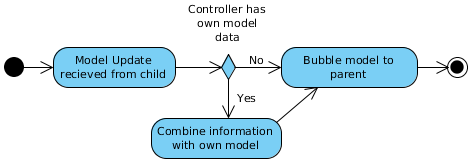
\includegraphics[scale=0.6]{../figures/authoring_tool/bubbling_to_root.png} 		
	\caption{\label{Figure: Bubbling to root} State diagram illustrating decisions when bubbling data to root} 	
\end{figure}

\autoref{Figure: Bubbling to root} demonstrates the decision making process to determine how the controller bubbles the data. Any controller that does not hold important model data will only bubble any information sent to it to the root controller. Any controller that has a model will also bubble its own model and model data received upwards. Therefore the global model is slowly accumulated by bubbling up the data. When it reaches the root controller the global model has been built and is saved for later use.

A controller holding model data stores the state of the controller which is represented by a HTML view. Each view is bound to its specific model using two way data binding. This means when the view is changed by the user the model will be automatically updated.

\begin{figure}[h]
	\centering
		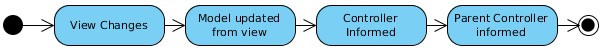
\includegraphics[scale=0.6]{../figures/authoring_tool/two_way_binding.png} 		
	\caption{\label{Figure: Authoring two way binding} Two way binding bubbling method illustrated in an state diagram} 	
\end{figure}

\autoref{Figure: Authoring two way binding} shows the process of the view changing and updating its parent. Each time the model is updated the controller runs any appropriate action to change the display of the view then sends the updated model to its parent. This change is bubbled upwards each level until it reaches the root controller who stores the new data in its global model.

\section{Conclusion}